\section{Руководство пользователя}
\label{sec:manual:intro}

\subsection{Руководство по разворачиванию приложения}
\label{sub:manual:deploy}

Приложения разрабатывалось с помощью package manager-а gradle, в котором прописаны все необходимые сторонние библиотеки, таким образом все нужный зависимости для проекта скачаются автоматически. Зависимости для UI собирались с помощь package manager-а npm, поэтому они так же скачаются автоматически, при сборке проекта.

Приложение использует следующие базы данных и сервисы:
\begin{itemize}
\item postgreSQL 9.3;
\item mongoDB 3.0;
\item redis 3.2;
\item rabbitMQ 3.6;
\item salesforce;
\item fullContact.
\end{itemize}

Всю конфигурацию для подключения баз данных и внешних сервисов, нужно прописывать в соответствующих файлах в git репозитории конфигурации:
\begin{itemize}
\item конфигурацию для подключению баз данных PostgreSQL, MongoDB, Redis, RabbitMQ в файле ets-service.yml;
\item конфигурацию для подключению Salesforce и с интегррованой с ним базой в файле salesforce-integration.yml;
\item конфигурацию для подключения сервиса предоставления публичной информации FullContact в файле social-integration.yml;
\item после того как соответствующая конфигурция будет прописана, нужно выполнить стандартные комманды git-а: git commit -а и git push.
\end{itemize}

После этого, чтобы собрать приложение нужно выполнить команду gradle build.

Если нужно запустить отдельный микросервис то его можно запустить соответствующей командой gradle :{microservice-name}:bootRun, где {microservice-name} имя микросервиса.

Для простоты разворачивания всех микросервисов сразу, был написан docker-compose.yml файл, с помощью которого одной командой docker-compose up, можно запустить все микросервисы сразу в docker контейнерах. Кроме того, он дает возможность легко горизонтально масштабировать отдельные микросервисы. 

Например: командой  docker-compose scale ets-service=5, поднимется 5 экземпляров микросервиса ets-service, и с помощью Ribbon другие микросервисы будут балансировать нагрузку по ним при обращении к сервису ets-service.

Для просмотра информации о развернутых серверов и их состояниях, можно зайти на {host:8761}, где host -- это адрес где развернут микросервис discovery-client (рисунок~\ref{fig:dc}).

\begin{figure}[h]
\centering
  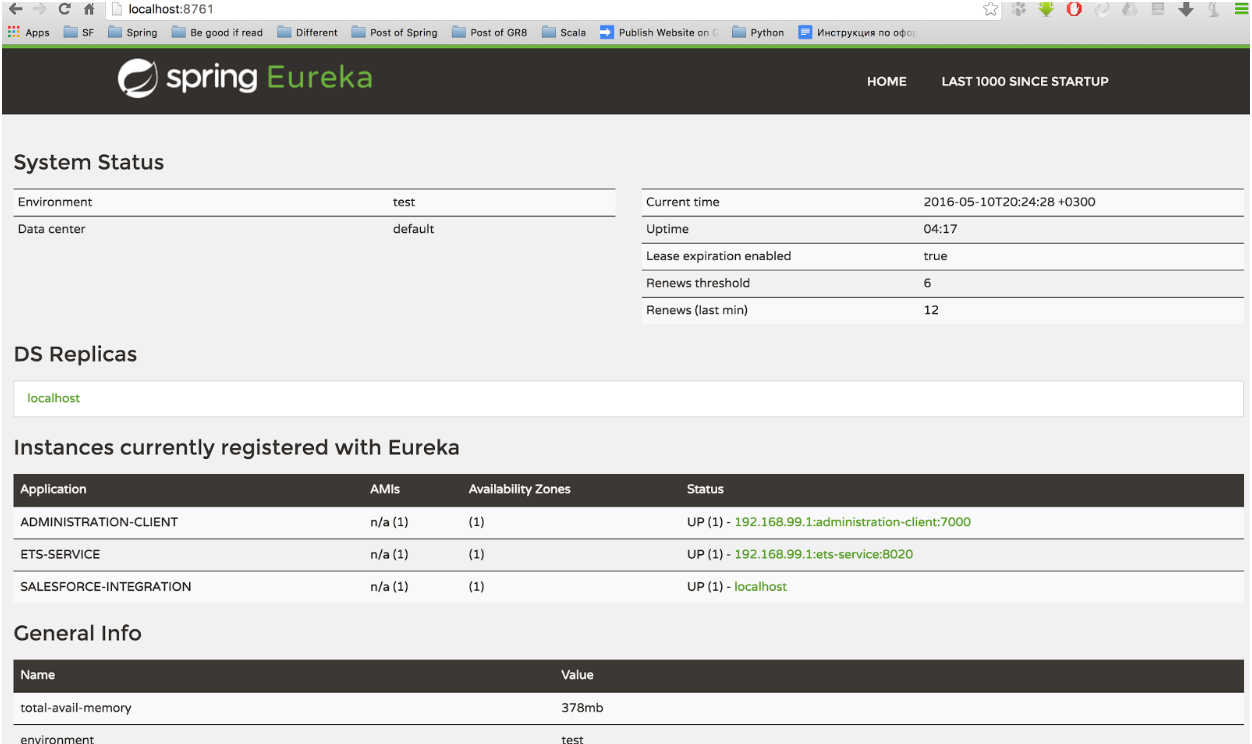
\includegraphics[scale=0.6]{dc.png}  
  \caption{Discovery client interface}
	\label{fig:dc}
\end{figure} 


\subsection{Руковоство для администраторов}
\label{sub:manual:admin}

В рамках данного проекта была также разработана панель администратора, в которой администраторы и менеджеры могут создавать/удалять/изменять и настраивать модели событий, которые будет поддерживать система, а так же возможность просмотра реал-тайм статистики происходящих событий. В рамках данной работы, постройка сложного UI не предполагалась, а наоборот цель была построить как можно более минималистический интерфейс, для проверки концепции архитектуры данной системы. 

На рисунке ~\ref{fig:events}, можно увидеть интерфейс на котором можно настраивать модели события под свои нужды.

\pagebreak
\begin{figure}[h]
\centering
  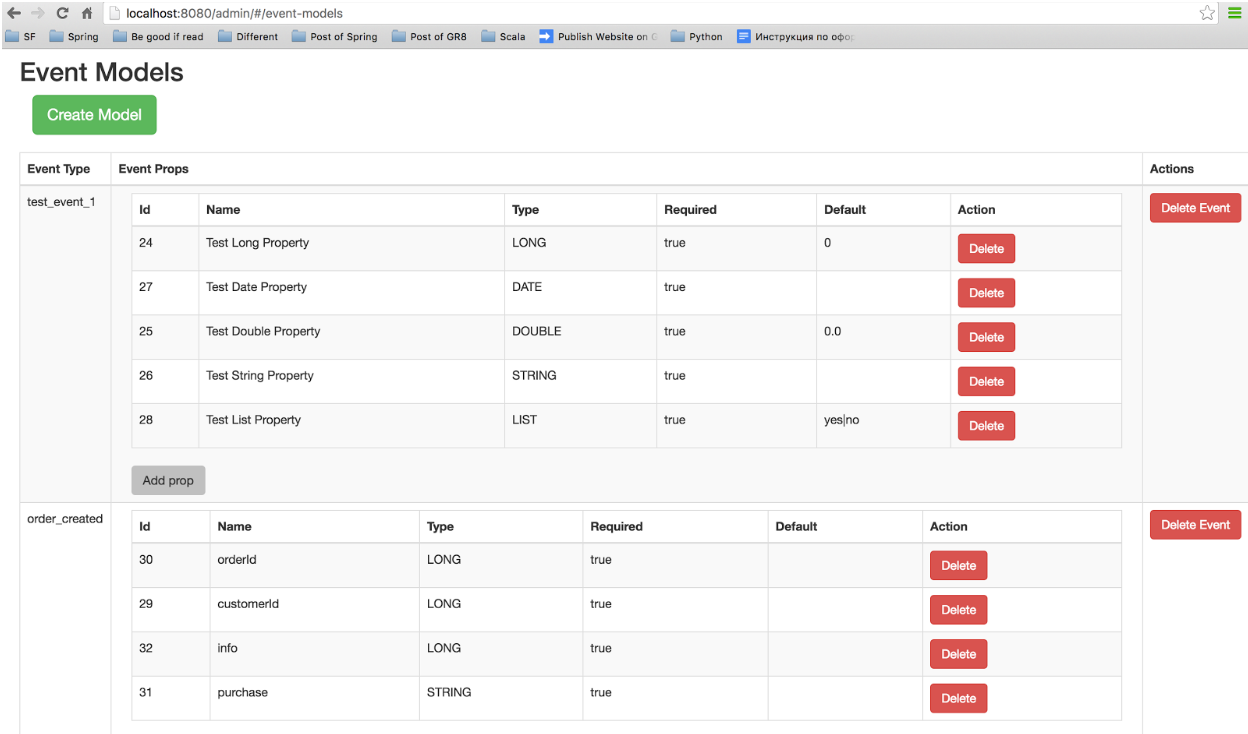
\includegraphics[scale=0.6]{events.png}  
  \caption{Интерфейс настройки моделей событий}
	\label{fig:events}
\end{figure}

На рисунке ~\ref{fig:event-prop} показано как выглядит интерфейс добавления и изменения того или иного поля в модели события.

\begin{figure}[h]
\centering
  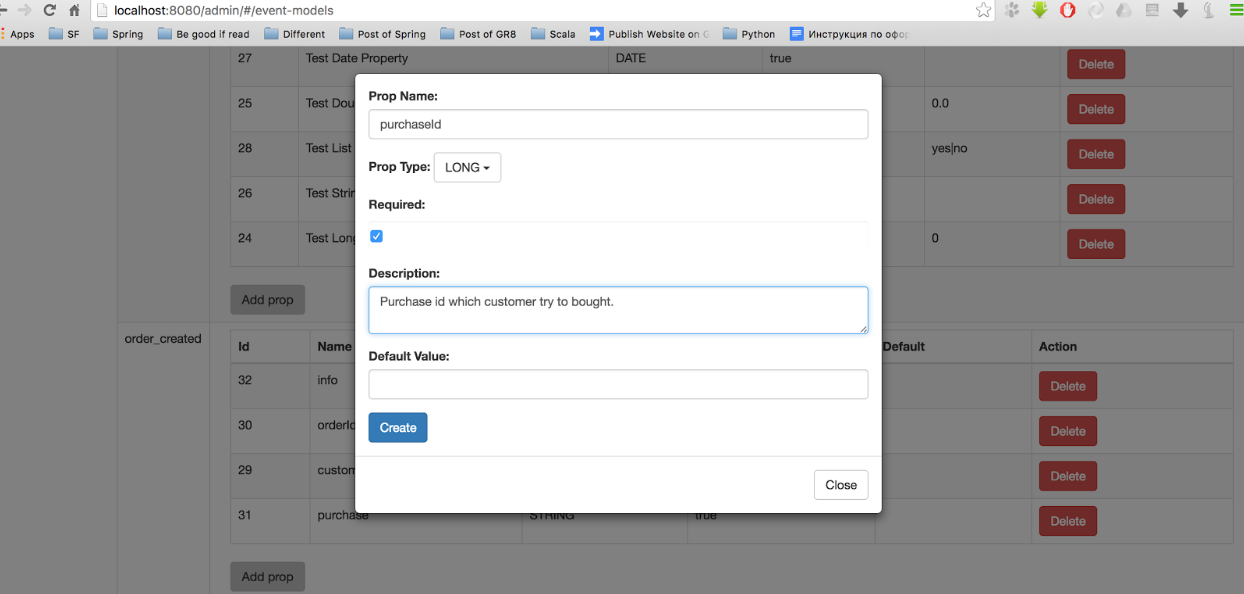
\includegraphics[scale=0.6]{event-prop.png}  
  \caption{Интерфейс настройки поля модели события}
	\label{fig:event-prop}
\end{figure}

Интерфейс просмотра статистики изображен на рисунке ~\ref{fig:stats}.
Так же на нем существует возможность просмотра статистики за определенный период. Для этого нужно всего ли выбрать соответствующий период.


\pagebreak
\begin{figure}[ht]
\centering
  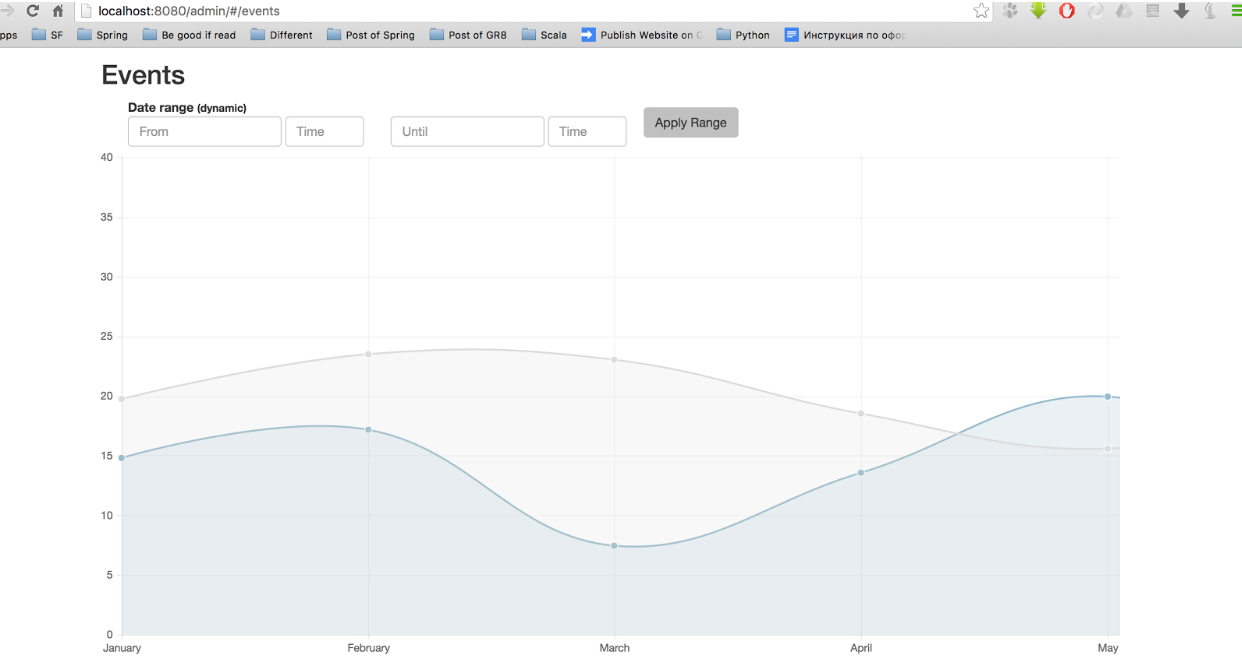
\includegraphics[scale=0.8]{stats.png}  
  \caption{Интерфейс просмотра статистики}
	\label{fig:stats}
\end{figure}

Наблюдать за состояниями микросервисов администраторы могут с помощью Hystrix Dashboard. Чтобы в него зайти нужно открыть страницу /hystrix-dashboard на которой будет поле для ввода источника данных для hystrix (https://hostname:port/turbine/turbine.stream).

На рисунке~\ref{fig:hystrix-m} изображен Hystrix Dashboard разрабатываемого программного средства.
\pagebreak
\begin{figure}[h]
\centering
  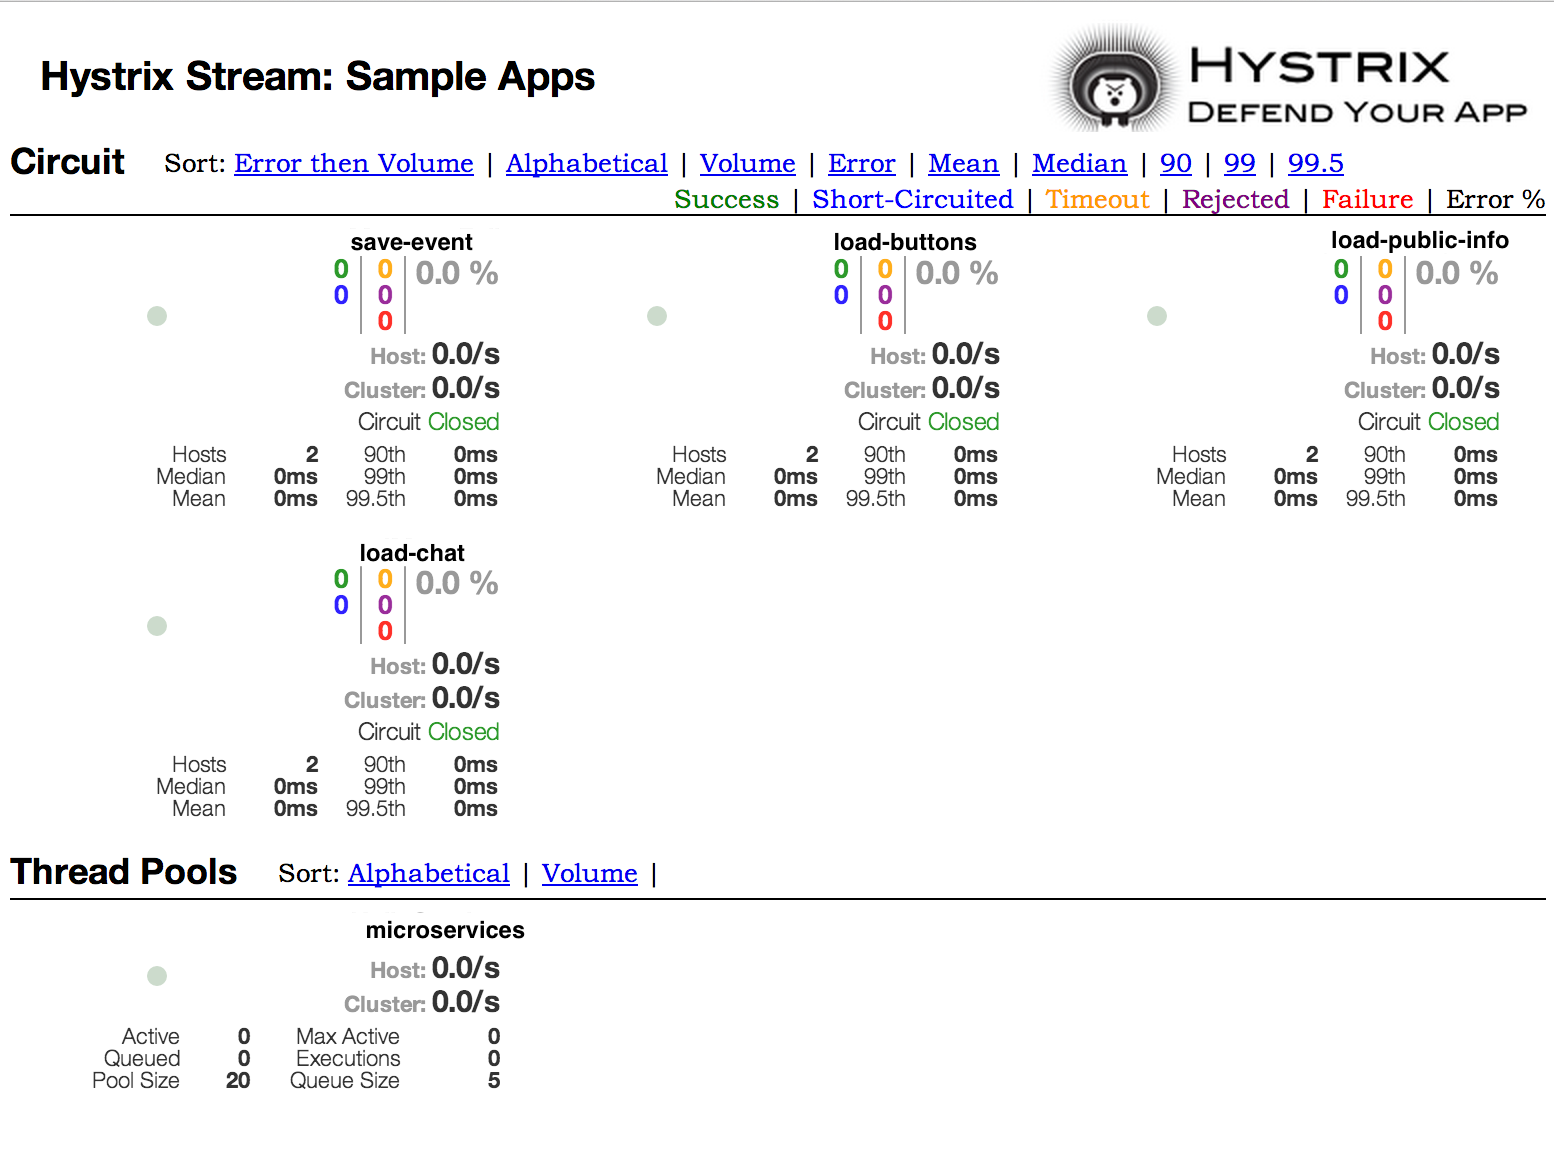
\includegraphics[scale=0.2]{hystrix.png}  
  \caption{Hystrix Dashboard программного средства}
  \label{fig:hystrix-m}
\end{figure} 



\subsection{Руководство по интеграции с онлайн чатом}
\label{sub:manual:chat}
На стороне salesforce есть множество настроек и критериев, по которым можно настроить онлайн чат под свои нужды. И в данный проект не подразумевает описание того как работает Salesforce. Подразумевается, что агенты которые будут общаться с посетителями через онлайн чат Salesforce, знаю его и умеют с ним работать. 
Со стороны агента чат будет как на рисунке ~\ref{fig:sf-chat}, также там предоставляются объекты Contact и Case в которых он заполняет, всё необходимую информацию собранную у клиента.

\begin{figure}[ht]
\centering
  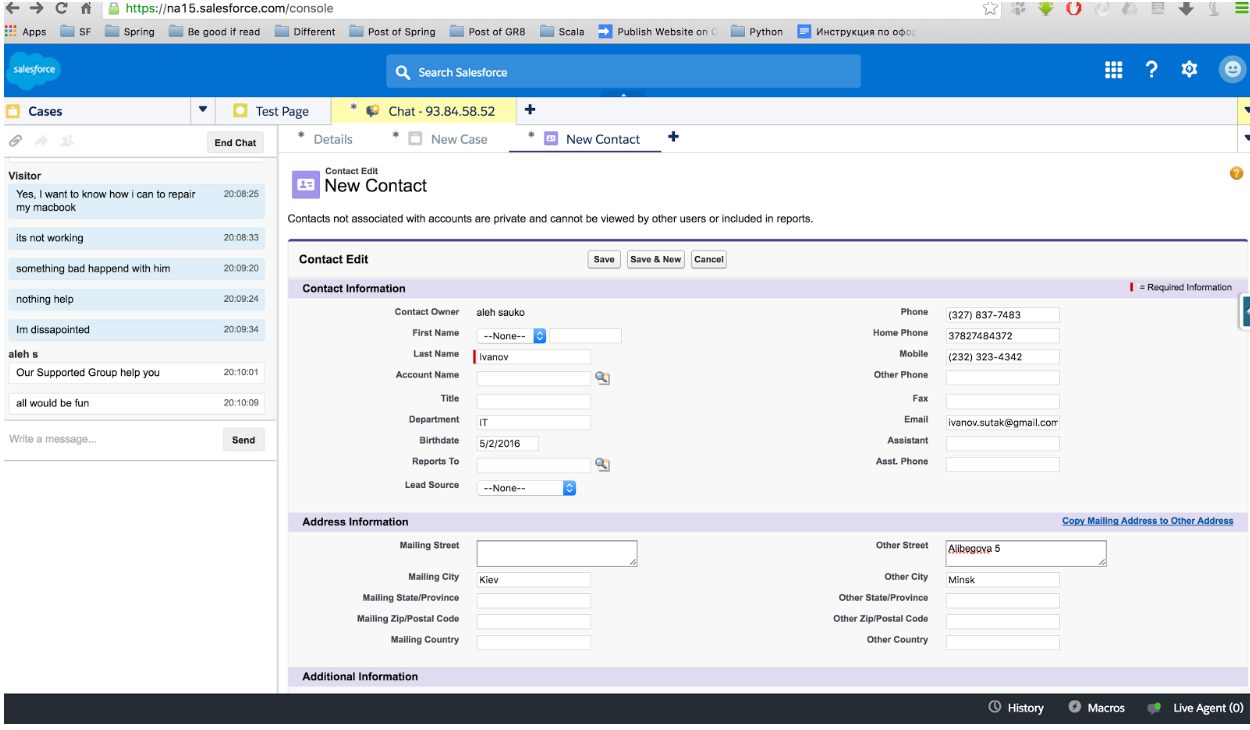
\includegraphics[scale=0.6]{sf-chat.png}  
  \caption{Salesforce online chat}
  \label{fig:sf-chat}
\end{figure}



\pagebreak
На стороне посетителя, чат выглядит как на рисунке ~\ref{fig:cl-chat}.

\begin{figure}[ht]
\centering
  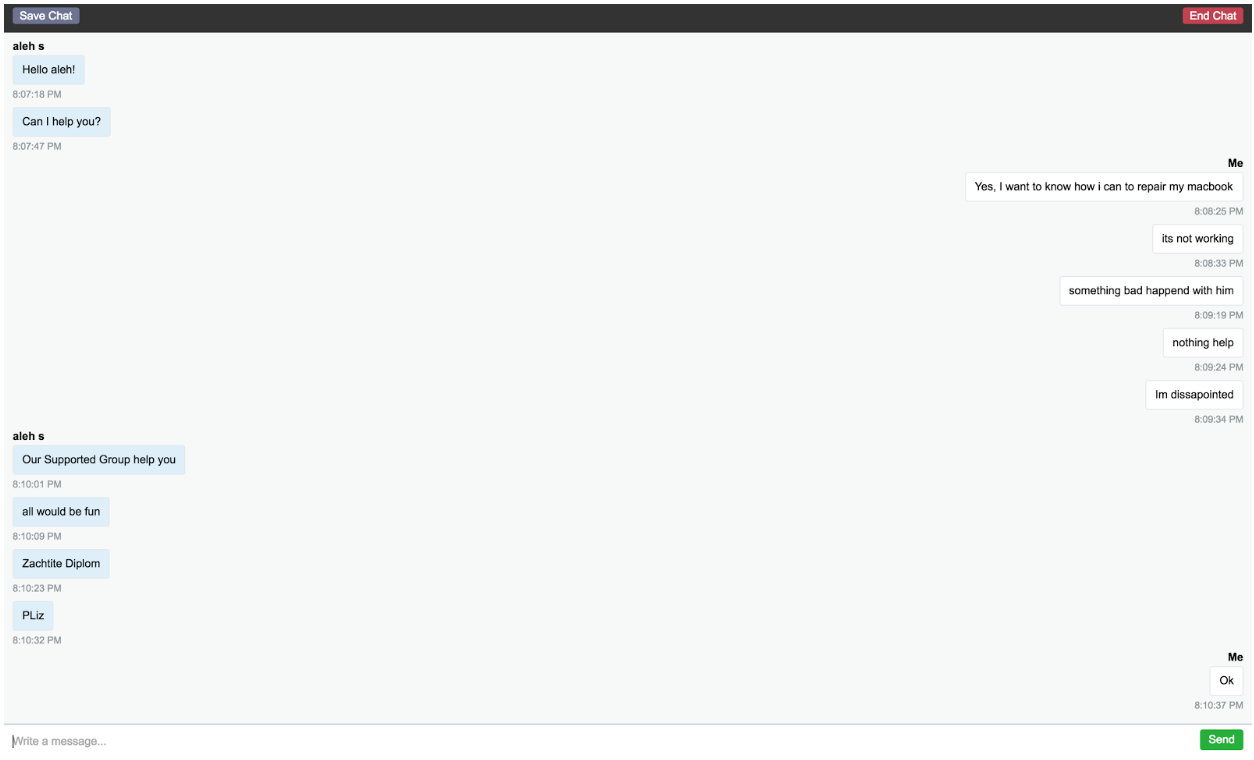
\includegraphics[scale=0.6]{cl-chat.png}  
  \caption{Client side chat}
  \label{fig:cl-chat}
\end{figure}